\documentclass[10pt,a4paper, twocolumn]{report}
\usepackage[utf8]{inputenc}
\usepackage[spanish]{babel}
\usepackage{amsmath}
\usepackage{amsfonts}
\usepackage{amssymb}
\usepackage{graphicx}
\author{Antonio Molina García-Retamero}
\title{Optimización de redes neuronales mediante métodos bioinspirados}
\makeindex
\begin{document}
\onecolumn
\maketitle
\pagebreak
\tableofcontents
\pagebreak
\twocolumn

\chapter{Introduction}
\section{Notas}
\begin{itemize}
	\item En Haykin, en el capítulo 10, habla de los modelos teóricos de información. Hay cosas chulas, con las que puedo apoyar la metaplasticidad
	 \item Además, en ese mismo capítulo, trata también de las gausianas sus propiedades. También la relación con la entropía del conocimiento a priori de los parámetros de la gausiana.
	 \item Entre las diferentes técnicas de entrenamiento de redes RBF, la técnica de las k-medias puede ser sustituida por otras con tal de evitar el tiempo de cómputo. Sin embargo, a partir de estas k-medias podemos acelerar el proceso de aprendizaje en el BP. Tal vez así conseguimos mejores resultado en tiempo similares.
\end{itemize}

\section{La metaplasticidad en redes biológicas}
\section{Metaplasticidad en redes neuronales artificiales}
\section{Trabajos previos}
\chapter{Metaplasticidad en Redes Neuronales con Función de Base Radial (RBFNN)}
\section{Estudio previo}
\section{La naturaleza stadística del proceso de aprendizaje}
\section{Refuerzo de casos menos frecuentes}
\section{Entrenamiento}
\chapter{Implementación}
\section{Metodología de desarrollo}
Aquí comento que he realizado la implementación siguiendo el paradigma TDD para la implementación de las redes.
\section{Pruebas y métricas de rendimiento}
Dado que por medio de este trabajo se pretende la demostración de la mejora propuesta sobre las RBFNN, estableceré en primer lugar una serie de pruebas que pretenderán poner a prueba las diferentes implementaciones de las redes para resolver problemas típicos.
La propuesta que aquí se presenta pretende mejorar el tiempo de aprendizaje haciendo del aprendizaje un proceso más eficiente reduciendo el error externo del sistema con un menor número de iteraciones. Es por esto que centraré el esfuerzo en mostrar como podemos acentuar la caída del error en el proceso de aprendizaje.
Sin embargo, para lograr esto repercutimos en un coste computacional que bien merece ser tenido en cuenta. Por ello también realizaré en paralelo pruebas que tengan por objeto mostrar como afecta la carga computacional extra e intentaré presentar escenarios en los que la mejora propuesta pueda suponer una mejora real.
De entre los escenarios en que las RBFNN se han caracterizado como herramientas especialmente útiles destacan el reconocimiento de patrones y los problemas de clasificación en los que se requieren de complejas transformaciiones no lineales para discernir entre clases.
Con todo esto en mente, he propuesto las siguientes pruebas que nos servirán para determinar los requerimientos del sistema a desarrollar:
\begin{itemize}
	\item Reconocimiento de patrones
	\begin{itemize}
		\item Onda compuesta
		\item Otra idea que se me ocurra
	\end{itemize}
	\item Clasificación
	\begin{itemize}
		\item Clasificador sobre datos artificiales
		\item Clasificador sobre datos estandarizados
	\end{itemize}
\end{itemize} 

\subsection{Pruebas de clasificación}
Uno de los usos más habituales de las RBFNN es cuando tenemos que clasificar sobre un conjunto de datos cuyas clases no son linealmente separables.
\begin{figure}[!h]{}
    \centering
    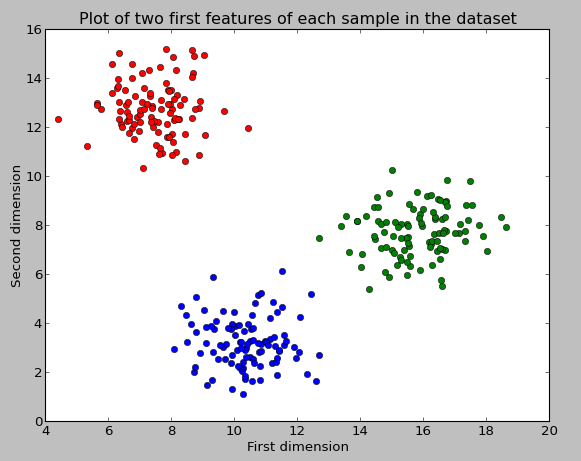
\includegraphics[width=0.4\textwidth]{img/clusteredData1.png}
    \label{fig:Suscripcion}
    \caption{Conjunto de datos con distribución normal}
\end{figure}
Ya que, a través de las RBFNN, obtenemos un modelo con la forma $f(x)=\sum w_{i}\phi(r)$ (que es caracterizado como funciones de base radial) podemos aproximar funciones complejas con gran precisión como podemos ver en la figura...
\section{Implementación básica de una RBF}

\section{Extendemos con centróides K-NN}
\section{PyBrain}


\chapter{Resultados}
\section{Resultados sobre las pruebas de rendimiento}
Como comentamos en la sección... 
\subsection{Pruebas de clasificación}
\section{Comparativa de RBFNN con y sin metaplasticidad}
\section{Otros resultados de interés}



\end{document}